\documentclass[mathserif]{beamer}
\mode<presentation>
{
  \usetheme{Frankfurt}
  \setbeamercovered{transparent}
}

\setbeamertemplate{caption}[numbered]

\usepackage{bm}
\usefonttheme[onlymath]{serif}
\usepackage{mathrsfs}

\begin{document}


\title{Learning to Communicate with Multi-Agents Reinforcement Learning}

\author{Wenhao Yang
}
\institute{School of Mathematical Sciences

Peking University}
\begin{frame}
  \titlepage
\end{frame}

\date{}

\begin{frame}{Outline}
\tableofcontents
\end{frame}
\section{Background}
\subsection{Deep Q-Networks}
\begin{frame}{Deep Q-Networks}
\begin{itemize}
  \item Aim: Single Agent
  \item Notation: state: $s_{t}$, action: $u_{t}$, reward: $r_{t}$, discout: $\gamma$,
  cumulative reward: $R_{t}=\sum_{k=0}^{\infty}r_{t+k}\gamma^{k}$
  \item Q-value function: $Q^{\pi}(s,u)=E[R_{t}|s_{t}=s,u_{t}=u]$
  \item Bellman equation: $Q^{*}(s,u)=E_{s'}[r+\gamma\max{u'}Q(s',u')|s,u]$
  \item Loss function: $L(\theta)=E[(r+\gamma\max_{u'}Q(s',u',\theta^{-})-Q(s,u,\theta))^{2}]$
\end{itemize}
\end{frame}
\subsection{Independent DQN}
\begin{frame}{Independent DQN}
\begin{itemize}
  \item Aim: Multi-Agents
  \item Settings:

  all observe global state

  Maximize team reward

  Each agents Q-value function: $Q^{a}(s,u^{a},\theta^{a})$
\end{itemize}
\end{frame}
\subsection{Deep recurrent Q-Networks}
\begin{frame}{Deep recurrent Q-Networks}
\begin{itemize}
  \item Only partial state $o_{t}$ is observed, global state $s_{t}$ is hidden

  \item Q(s,u) can't be approximated as $s$ is not known

  \item Solution: Approximate $Q(o_{t},h_{t-1},u)$ with recurrent network,
  where $h_{t}$ represents the hidden state of the network

\end{itemize}
\end{frame}
\section{Models}
\begin{frame}{Setting}
  \begin{itemize}
    \item Consider Multi-Agents and partially observation
    \item Maximize team reward
    \item Each agent receives $o_{t}^{a}$ correlated to $s_{t}$
    \item In each time-step, agents select an environment action $u\in U$
    and a communication action $m\in M$
    \item Communication action is observed by other agents but has no
    direct impact on the environment or reward
    \item Parameters sharing
  \end{itemize}
\end{frame}
\subsection{Reinforced Inter-Agent Learning(RIAL)}
\begin{frame}{Reinforced Inter-Agent Learning(RIAL)}
\begin{itemize}
  \item Deep Recurrent Q-network and independent Q-learning
  \item Q-value: $Q^{a}(o_{t}^{a},m_{t-1}^{a'},h_{t-1}^{a},u^{a})$
  \item Structure:
  \begin{figure}
    \centering
    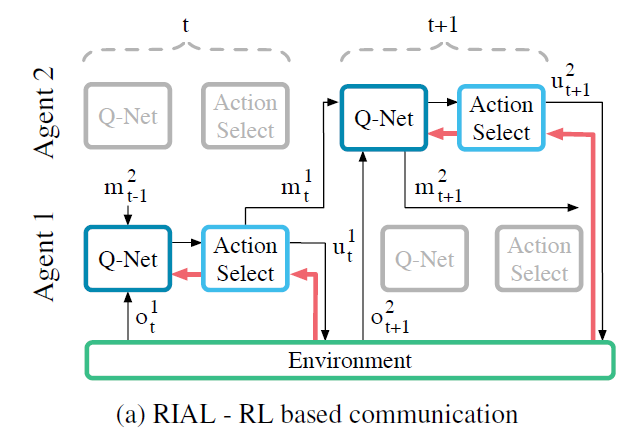
\includegraphics[scale=0.6]{fig/1}
  \end{figure}
\end{itemize}
\end{frame}
\subsection{Differentiable Inter-Agent Learning(DIAL)}
\begin{frame}{Differentiable Inter-Agent Learning(DIAL)}
  \begin{itemize}
    \item Feedback about communication actions
    \item Structure:
    \begin{figure}
      \centering
      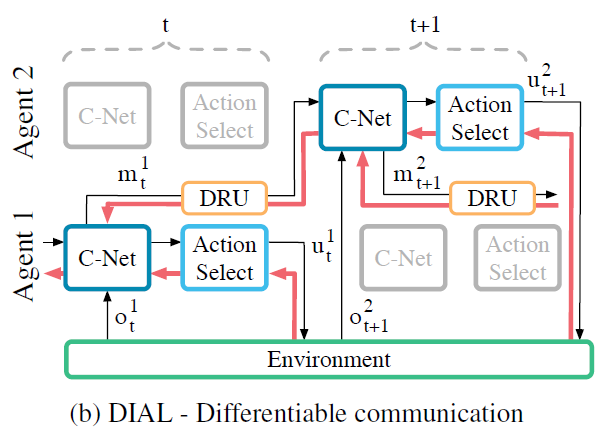
\includegraphics[scale=0.6]{fig/2}
    \end{figure}
  \end{itemize}
\end{frame}

\begin{frame}{Model Architecture}
  \begin{figure}
    \centering
    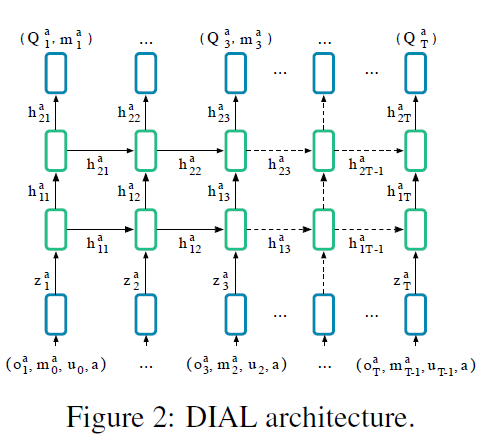
\includegraphics[scale=1]{fig/3}
  \end{figure}
\end{frame}

\begin{frame}{Model Architecture}
  \begin{itemize}
    \item Input: $(o_{t}^{a},m_{t-1}^{a'},u_{t-1}^{a},a)$
    \item Embedding:

    $z_{t}^{a}=f_{1}(o_{t}^{a})+f_{2}(m_{t-1})+f_{3}(u_{t-1}^{a})+f_{4}(a)$

    where $f_{1}$ is a task-specific network, $f_{2}$ is a 1-layer MLP and
    $f_{3}$ and $f_{4}$ are lookup tables
    \item 2-layer RNN with GRUs
    \item Output: $Q_{t}^{a},m_{t}^{a}$
  \end{itemize}
\end{frame}

\begin{frame}{Algorithm(DIAL)}
\begin{figure}'
  '
  \centering
  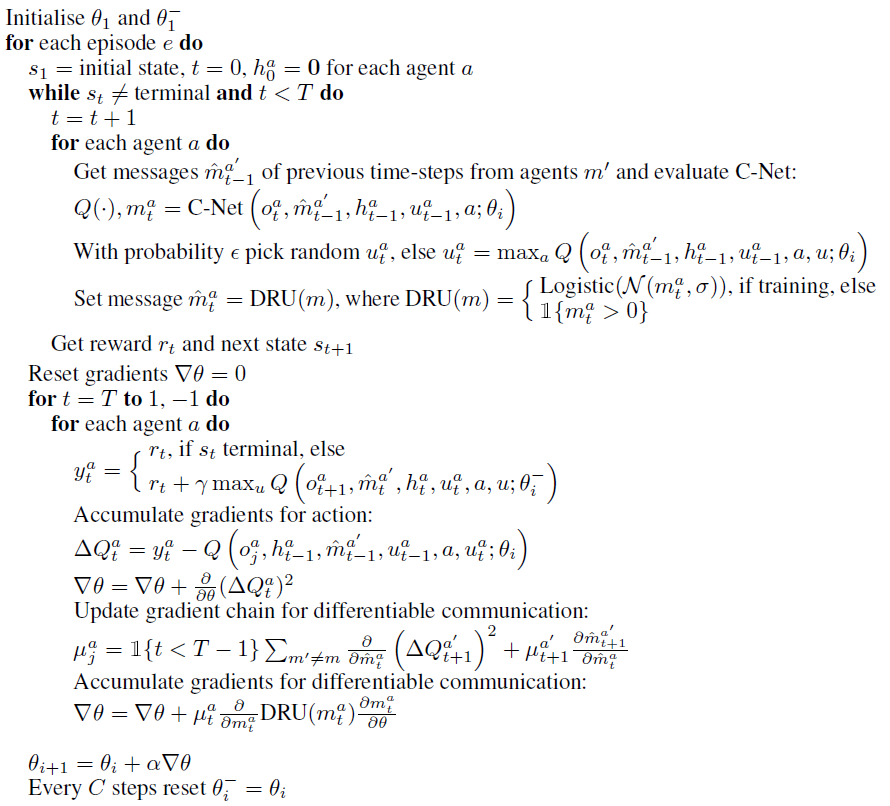
\includegraphics[scale=0.5]{fig/4}
\end{figure}
\end{frame}
\section{Experiments}
\subsection{Switch Riddle}
\begin{frame}{Experiment: Switch Riddle}
  \begin{figure}
    \centering
    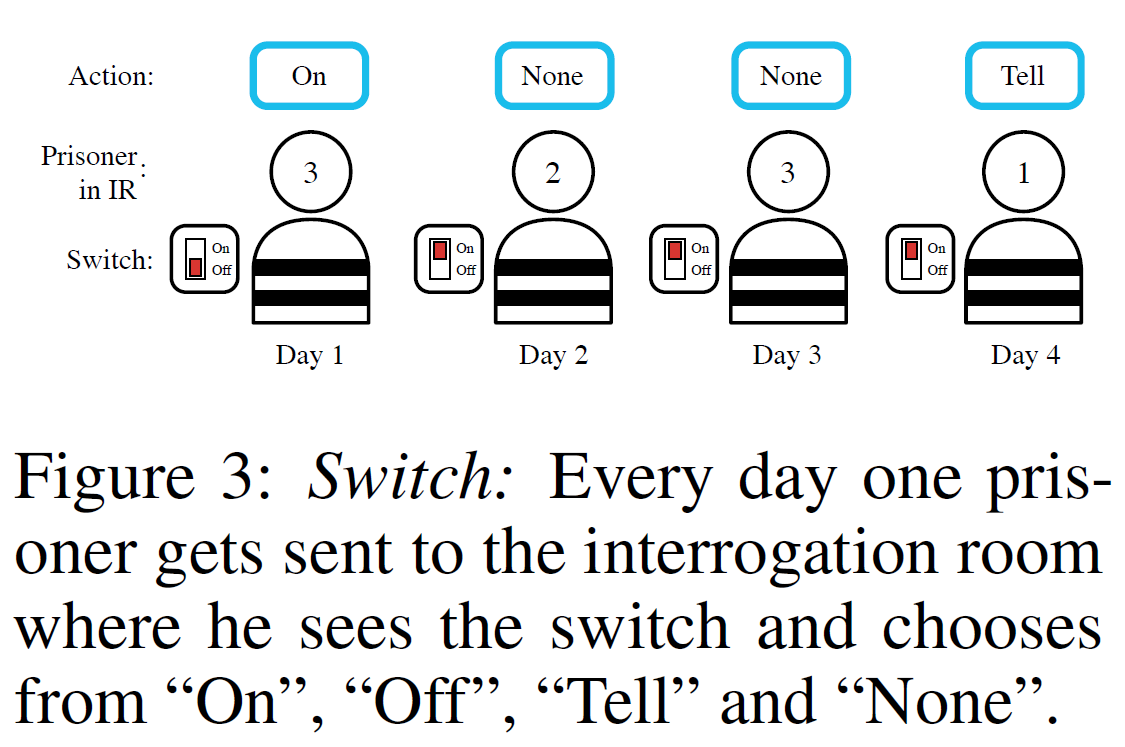
\includegraphics[scale=0.5]{fig/5}
  \end{figure}
\end{frame}

\begin{frame}{Experiment: Switch Riddle}
  \begin{itemize}
    \item $m_{t}^{a},o_{t}^{a}\in\{0,1\}$
    \item $u_{t}^{a}\in\{None,Tell\}$
    \item $r_{t}\in\{-1,0,1\}$
    \item Results:
    \begin{figure}
      \centering
      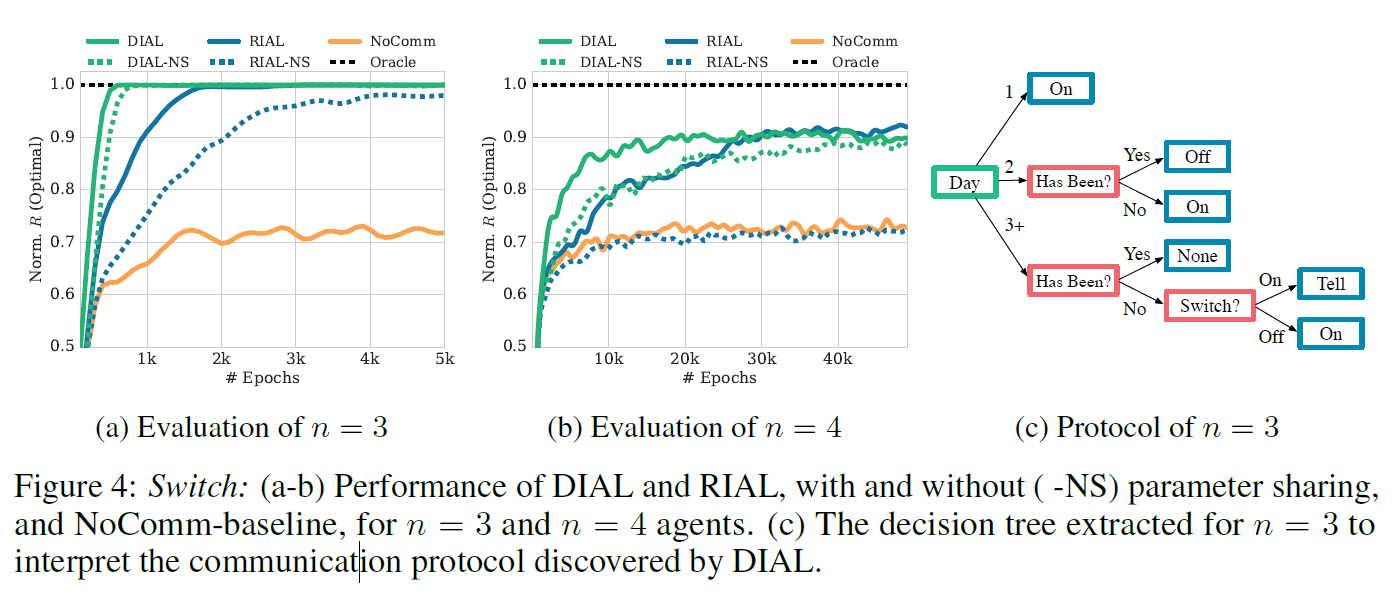
\includegraphics[scale=0.4]{fig/6}
    \end{figure}
  \end{itemize}
\end{frame}
\subsection{Multi-Step MNIST}
\begin{frame}{Experiment: Multi-Step MNIST}
  \begin{figure}
    \centering
    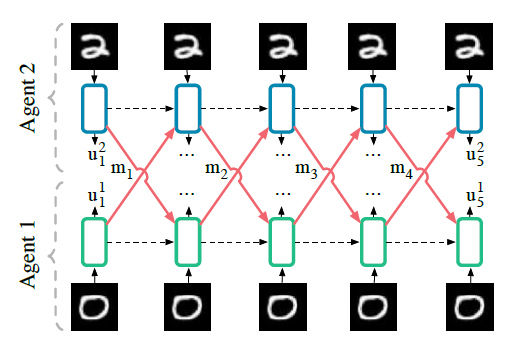
\includegraphics[scale=0.8]{fig/8}
  \end{figure}
\end{frame}
\subsection{Colour-Digit MNIST}
\begin{frame}{Experiment: Colour-Digit MNIST}
  \begin{figure}
    \centering
    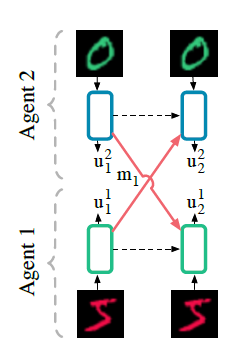
\includegraphics[scale=0.8]{fig/7}
  \end{figure}
  Not descriped clearly in paper
\end{frame}
\begin{frame}{MNIST results}
  \begin{figure}
    \centering
    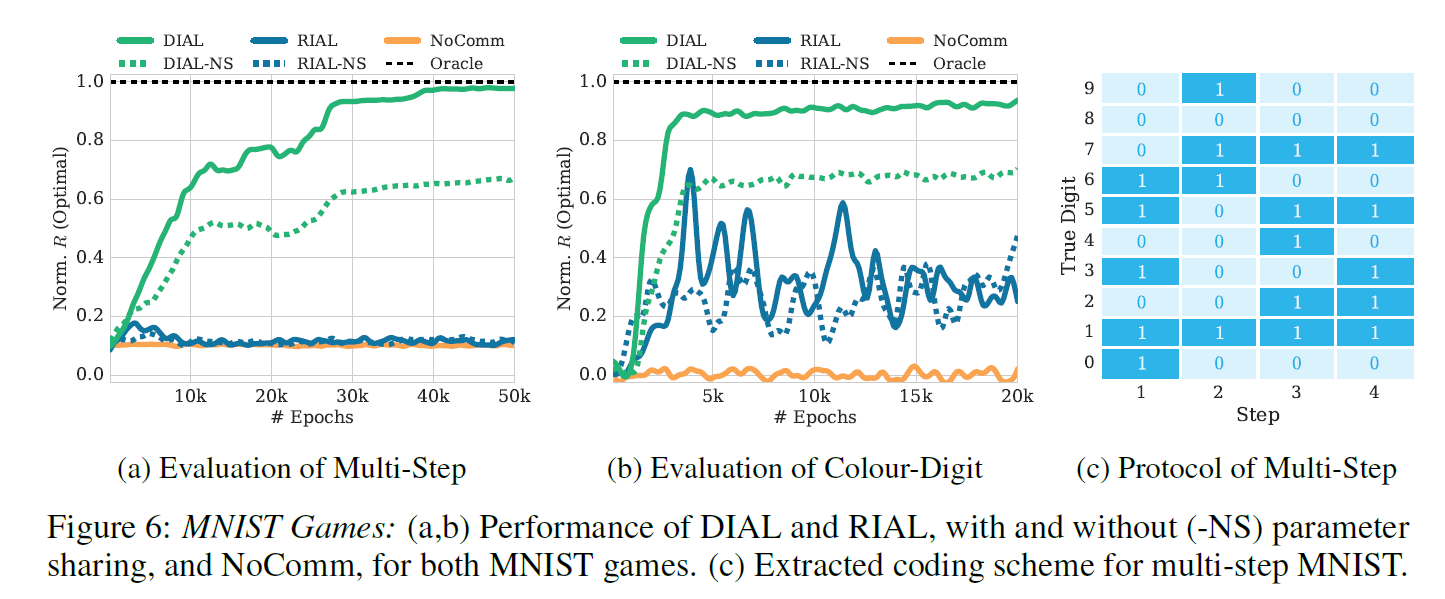
\includegraphics[scale=0.4]{fig/9}
  \end{figure}
\end{frame}
\section{Reference}
\begin{frame}{Reference}
  Reference:

  [1] Jakob N. Foerster, Yannis M. Assael, Nando de Freitas, Shimon Whiteson; Learning to Communicate with Deep Multi-Agent Reinforcement Learning
\end{frame}
\end{document}
